%=======================02-713 LaTeX template, following the 15-210 template==================
%
% You don't need to use LaTeX or this template, but you must turn your homework in as
% a typeset PDF somehow.
%
% How to use:
%    1. Update your information in section "A" below
%    2. Write your answers in section "B" below. Precede answers for all 
%       parts of a question with the command "\question{n}{desc}" where n is
%       the question number and "desc" is a short, one-line description of 
%       the problem. There is no need to restate the problem.
%    3. If a question has multiple parts, precede the answer to part x with the
%       command "\part{x}".
%    4. If a problem asks you to design an algorithm, use the commands
%       \algorithm, \correctness, \runtime to precede your discussion of the 1
%       description of the algorithm, its correctness, and its running time, respectively.
%    5. You can include graphics by using the command \includegraphics{FILENAME}
%
\documentclass[11pt]{article}
\usepackage{amsmath,amssymb,amsthm}
\usepackage{graphicx}
\usepackage[margin=1in]{geometry}
\usepackage{fancyhdr}
\setlength{\parindent}{0pt}
\setlength{\parskip}{5pt plus 1pt}
\setlength{\headheight}{13.6pt}
\newcommand\question[2]{\vspace{.25in}\hrule\textbf{#1: #2}\vspace{.5em}\hrule\vspace{.10in}}
\renewcommand\part[1]{\vspace{.10in}\textbf{(#1)}}
\newcommand\algorithm{\vspace{.10in}\textbf{Algorithm: }}
\newcommand\correctness{\vspace{.10in}\textbf{Correctness: }}
\newcommand\runtime{\vspace{.10in}\textbf{Running time: }}
\pagestyle{fancyplain}
\lhead{\textbf{\NAME\ (\ANDREWID)}}
\chead{\textbf{Assignment \HWNUM - Splines}}
\rhead{\today}

\usepackage{IEEEtrantools}
\usepackage{listings}
\usepackage{caption}
\usepackage{subcaption}
\usepackage{subfig}
\usepackage{wrapfig,lipsum,booktabs}

% Python style for highlighting
\newcommand\pythonstyle{\lstset{
language=Python,
basicstyle=\ttm,
otherkeywords={self},             % Add keywords here
keywordstyle=\ttb\color{deepblue},
emph={MyClass,__init__},          % Custom highlighting
emphstyle=\ttb\color{deepred},    % Custom highlighting style
stringstyle=\color{deepgreen},
frame=tb,                         % Any extra options here
showstringspaces=false            % 
}}


% Python environment
\lstnewenvironment{python}[1][]
{
\pythonstyle
\lstset{#1}
}
{}

\begin{document}\raggedright
%Section A==============Change the values below to match your information==================
\newcommand\NAME{Surajkumar H}  % your name
\newcommand\ANDREWID{EE11B075}     % your andrew id
\newcommand\HWNUM{2}              % the homework number
%Section B==============Put your answers to the questions below here=======================

% no need to restate the problem --- the graders know which problem is which,
% but replacing "The First Problem" with a short phrase will help you remember
% which problem this is when you read over your homeworks to study.

\question{1}{Questions 1 \& 2: Intro to Splines} 
\setcounter{section}{1}
For Questions 1-7, we deal primarily with the function given by 
\begin{equation}
f(x) = \frac{x^{1+J_0(x)}}{\sqrt{(1+100x^2)(1-x)}} = \frac{x^{1+J_0(x)}}{\sqrt{1-x+100x^2-100x^3}} 
\label{func}
\end{equation}

We perform various schemes of spline interpolation (not-a-knot, clamped) considering uniform spacing of the points. We also observe how incorrectly specifying the end derivative value  causes the error to blow up, and use this to gain insight into the spline algorithm.

We then come up with a non-uniform point spacing scheme which uses the (almost) minimum number of points to achieve 6-digit accuracy. We then compare the performance spline interpolation and rational interpolation in fitting this particular function.



\subsection{Background}

Spline interpolation uses the knowledge of the function derivatives to fit a smooth polynomial function between points. We focus in particular on the cubic spline, which uses the 2nd-derivatives to fit a cubic polynomial. This ensures that the 2nd-derivative is continuous throughout the domain. 


Say the cubic spline interpolated value at $x$ is given by some $y$. We find the nearest 2 points, say $x_{j}$, and $x_{j+1}$. Let the function values at these points be $y_{j}$ and $y_{j+1}$, and let the 2nd-derivative values be $y_{j}''$ and $y_{j+1}''$. The interpolated value $y$ is given by,
\begin{equation}
y=Ay_{j}+By_{j+1}+Cy_{j}''+Dy_{j+1}''
\end{equation}
where $A$ and $B$ are given as 
\begin{equation}
A=\frac{x_{j+1}-x}{x_{j+1}-x_{j}} \:\:\:\:\:\:\:\:\:\:\:\:\:\:\:\: B=\frac{x-x_{j}}{x_{j+1}-x_{j}}
\end{equation}
and the 2nd-derivative coefficients $C$ and $D$ are given by
\begin{equation}
C=\frac{1}{6}(A^3-A)(x_{j+1}-x_{j})^2 \:\:\:\:\:\:\:\:\:\:\:\:\:\:\:\: D=\frac{1}{6}(B^3-B)(x_{j+1}-x_{j})^2
\end{equation}

Using these, we can obtain expressions for the first and second derivative of $y$.
\begin{equation}
   \frac{dy}{dx} = \frac{y_{j+1}-y_{j}}{x_{j+1}-x_{j}} - \frac{3A^2-1}{6}(x_{j+1}-x_{j})y_{j}'' + \frac{3B^2-1}{6}(x_{j+1}-x_{j})y_{j+1}''
   \label{deriv1}
   \end{equation}   
\begin{equation}
\frac{d^2y}{dx^2} = Ay_{j}'' + By_{j+1}''
\end{equation}
which ensures that the interpolation is Lagrangian in both the function values and the 2nd-derivative. This ensures that the values at the data points are exactly matched. 

We assume knowledge of the 2nd-derivative while performing cubic-spline interpolation. To obtain these, we further stipulate continuity of the 1st-derivatives across the interval boundaries. We do this by using the neighbouring sets of points $(x_{j-1},x_{j})$ and $(x_{j},x_{j+1})$ in (\ref{deriv1}). This gives us the condition (for $j=2,3,\ldots,N-1$)
\begin{equation}
\frac{x_{j}-x_{j-1}}{6}y_{j-1}'' + \frac{x_{j+1}-x_{j-1}}{3}y_{j}'' + \frac{x_{j+1}-x_{j}}{6}y_{j}'' = \frac{y_{j+1}-y_{j}}{x_{j+1}-x_{j}} - \frac{y_{j}-y_{j-1}}{x_{j}-x_{j-1}}
\end{equation}

This gives us $N-2$ linear equations in the $N$ unknowns $y_{1}'',y_{2}'',\ldots,y_{N}''$. We need 2 more equations to solve for the 2nd-derivatives. We use various boundary conditions as the other 2 equations. Depending on the nature of equations we use, we get different types of cubic splines. These are:
\begin{itemize}
\item \textbf{Normal Spline} - The second derivatives are zero at the ends.

\item \textbf{Clamped Spline} - The first derivative of the function is specified at the end points. This translates to setting (\ref{deriv1}) to a given value. 
\begin{equation}
\begin{split}
\frac{y_{2}-y_{1}}{x_{2}-x_{1}} - \frac{1}{3}(x_{2}-x_{1})y_{1}'' - \frac{1}{6}(x_{2}-x_{1})y_2'' &= y_1' \\
\frac{y_{N}-y_{N-1}}{x_{N}-x_{N-1}} - \frac{1}{6}(x_{N}-x_{N-1})y_{N-1}'' - \frac{1}{3}(x_{N}-x_{N-1})y_{N}'' &=y_N'
\end{split}
\end{equation}
\item \textbf{Not-a-Knot spline} - Without specifying any extra conditions at the end points, the not-a-knot spline requires that the 3rd-derivative of the spline is continuous at $x_2$ and $x_{N-1}$. We can derive these conditions to be 
\begin{equation}
\begin{split}
(x_3-x_2)y_1'' - (x_3-x_1)y_2'' + (x_2-x_1)y_3'' &= 0 \\
(x_N-x_{N-1})y_{N-2}'' - (x_3-x_{N-2})y_{N-1}'' + (x_{N-1}-x_{N-2})y_N'' &= 0
\end{split}
\end{equation}
\end{itemize}

We prefer not-a-knot spline if there is no prior knowledge of the function derivatives, as this ensures maximal smoothness. We use the base \textsc{spline.c} code for the cubic spline interpolation.

\subsection{Function Plot}

The plot of the function $f(x)$ given by (\ref{func}) over $[0.1,0.9]$ is shown in Figure \ref{q1:func}. The function takes $0$ value at $x=0$ and goes to $\infty$ as $x \to 1$. The function is analytic in $[0,1)$


\begin{figure}
\centering
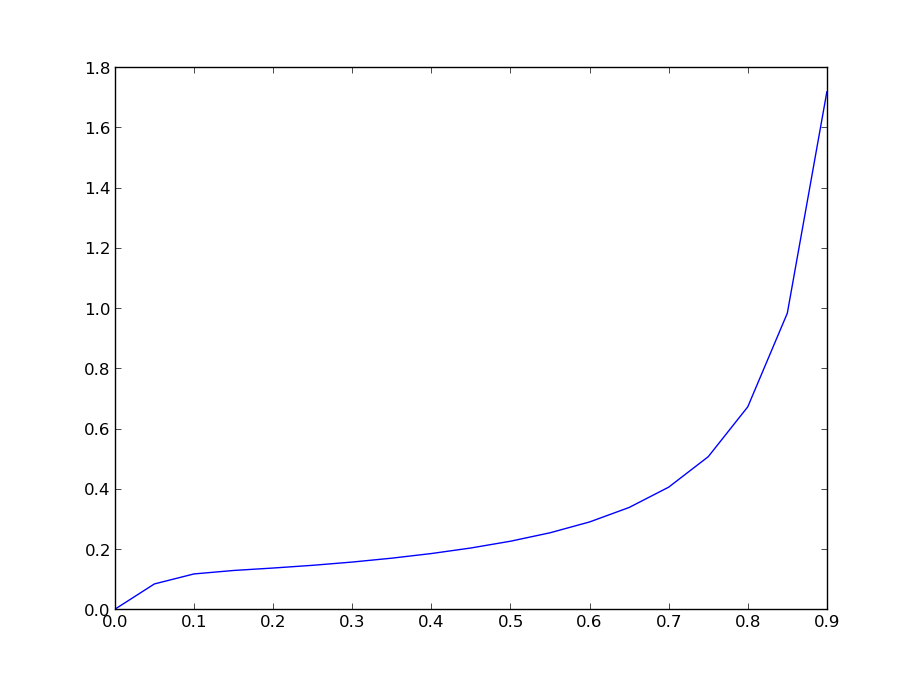
\includegraphics[width=0.5\linewidth]{q1-q2/func.png}
\caption{Function plot $f(x)$}
\label{q1:func}
\end{figure}

\question{4}{Question 4: Clamped Splines} 
\setcounter{section}{4}

\begin{figure*}
        \centering
        \begin{subfigure}{.5\textwidth}
  \centering
        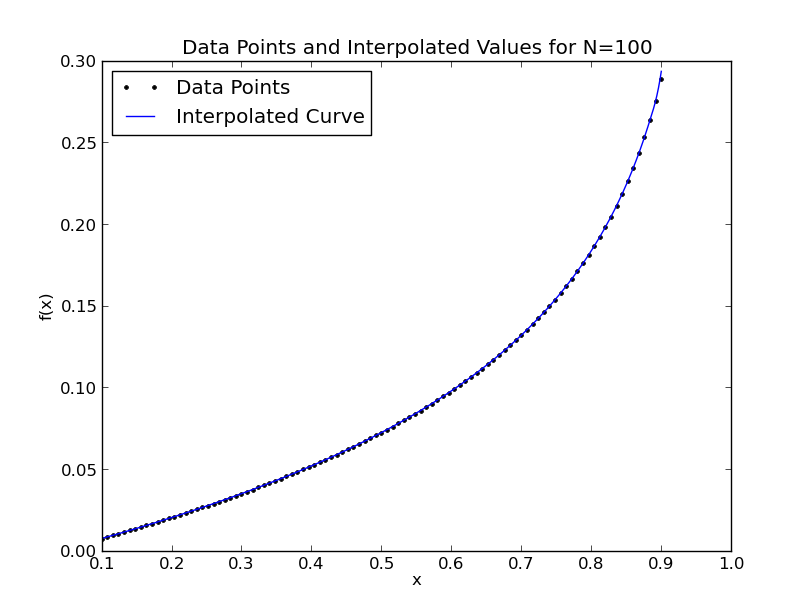
\includegraphics[width=\linewidth]{q4/func_low.png}
                \caption{Theoretical and interpolated values of $f(x)$}
                \label{fig:q4_1_func}
                \end{subfigure}%
\begin{subfigure}{.5\textwidth}
  \centering
        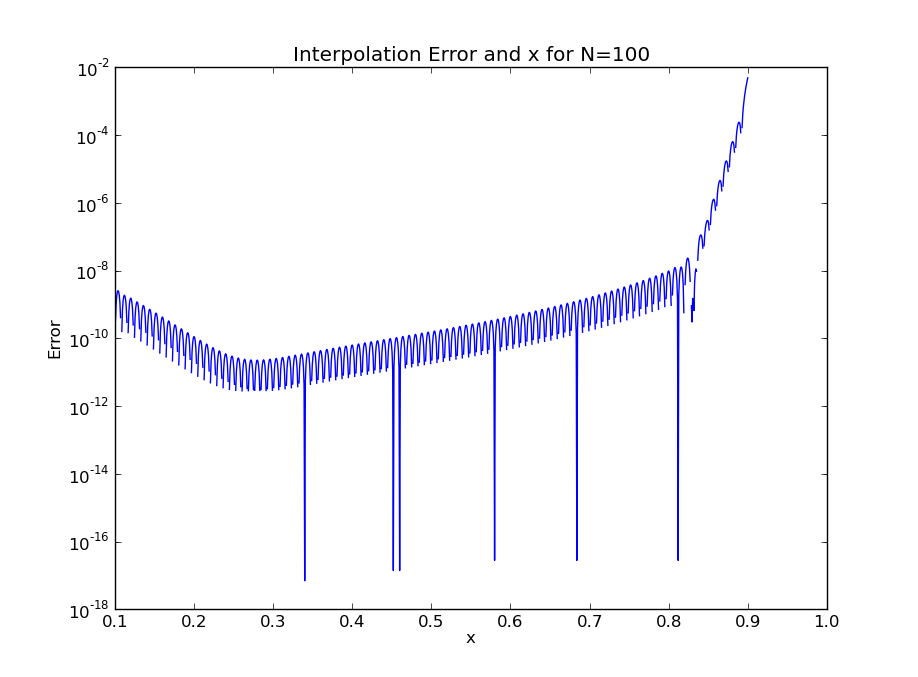
\includegraphics[width=\linewidth]{q4/err_low_2.png}
                \caption{Spline Interpolation Error for $N=100$}
                \label{fig:q4_1_err}
	\end{subfigure}
            
\caption{Cubic Spline Interpolation using $N=100$, function plot and error. }
\label{fig:q4_1}            
\end{figure*}

In this question, we evaluate the performance of spline interpolation when the derivative at the end points are specified. We also observe the effect of varying point spacing on interpolation error, find the first 6 digit accurate interpolation scheme, and observe how the error evolves with point spacing. Giving more information can potentially improve the performance of the algorithm. We analytically compute the value of the first derivative at $x=0.1,0.9$, and pass this to the \textsc{spline} function. We define \textsc{func deriv} to compute the derivative value at these points. To do this, we let $N(x)=x^{1+J_0(x)}$ and $D(x)=\sqrt{1-x+100x^2-100x^3}$. Then $f(x)=\frac{N(x)}{D(x)}$. We can then evaluate $f'(x)$ as, 

\begin{IEEEeqnarray}{rCl}
N'(x) &=& x^{1+J_0(x)} \left( -J_1(x)log(x) + \frac{1+J_0(x)}{x} \right) \nonumber \\
D'(x) &=& \frac{-1+200x-300x^2}{2\sqrt{1-x+100x^2-100x^3}} \nonumber \\
f'(x) &=& \frac{D(x)N'(x) - N(x)D'(x)}{(D(x))^2}
\end{IEEEeqnarray}

Using this, we perform spline interpolation. We use \textsc{logspace} to systematically vary up with the spacing of sample points. Figures (\ref{fig:q4_1_func}) and (\ref{fig:q4_1_err}) show the interpolation for $N=100$ points uniformly spaced in $[0.1,0.9]$. We see that the error blows up as $x\to 0.9$, as we get closer to the singularity. 

We see that the first 6-digit accurate interpolation scheme uses $N=8483$. This means that the point spacing $\Delta x < 10^{-4}$. We see from Figure (\ref{fig:q4_2_err}) that the error is low over most fo the interval, but shoots up near the singularity. The high point spacing just ensures that the shoot up still maintains 6-digit accuracy. Figure (\ref{fig:q4_2_loglog}), shows how the max interpolation error decreases almost linearly with number of data points ($loglog$ scale). So, $Err \propto \frac{1}{(No\;of\;Points)^\alpha}$

\begin{figure*}
        \centering
        \begin{subfigure}{.5\textwidth}
  \centering
        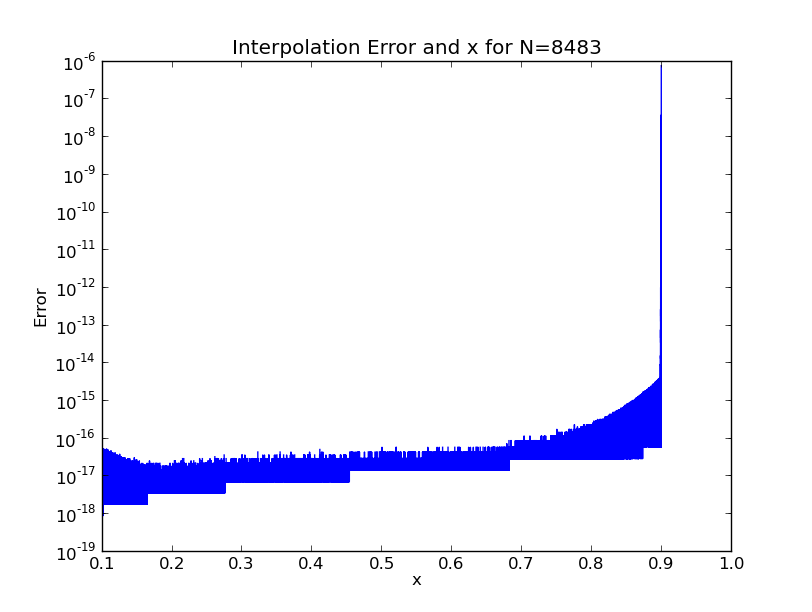
\includegraphics[width=\linewidth]{q4/err_high.png}
                \caption{Spline Interpolation Error for $N=8483$}
                \label{fig:q4_2_err}
                \end{subfigure}%
\begin{subfigure}{.5\textwidth}
  \centering
        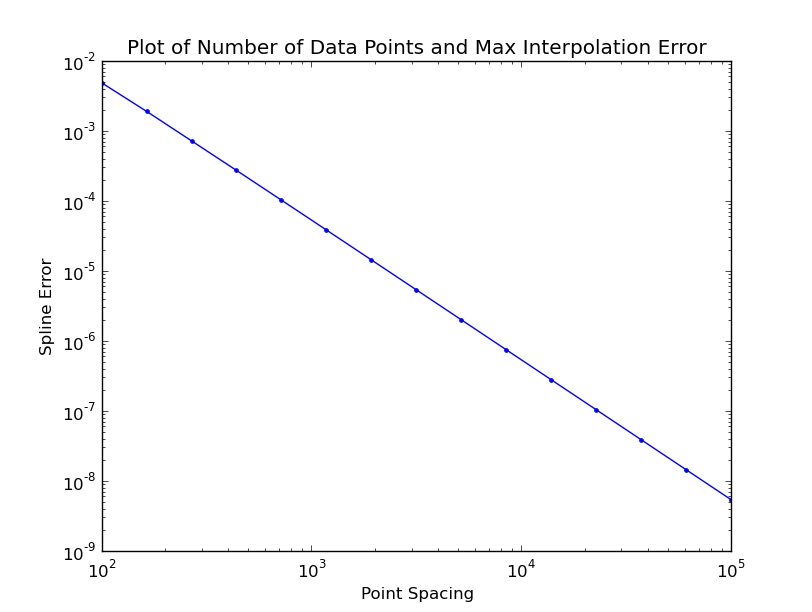
\includegraphics[width=\linewidth]{q4/loglogerr.png}
                \caption{Variation of Interpolation Error with Spacing}
                \label{fig:q4_2_loglog}
	\end{subfigure}
            
\caption{Cubic Spline Interpolation using $N=100$, function plot and error. }
\label{fig:q4_2}            
\end{figure*}

\question{5}{Questions 5: Giving a different derivative } 
\setcounter{section}{5}

In this question, we evaluate the performance of the clamped spline algorithm when the end point derivatives are incorrectly specified. This is of tremendous importance, since we might not actually know the derivatives, or might make approximations. Ideally, we want our algorithm to do reasonably well under derivative change. It is evident that the interpolation will take a hit near the end points, but we would ideally like the intermediate interpolation error to be more or less the same. This goes back to the stability arguments of the Spline algorithm. 


\begin{figure*}[h]
        \centering
        \begin{subfigure}{.5\textwidth}
  \centering
        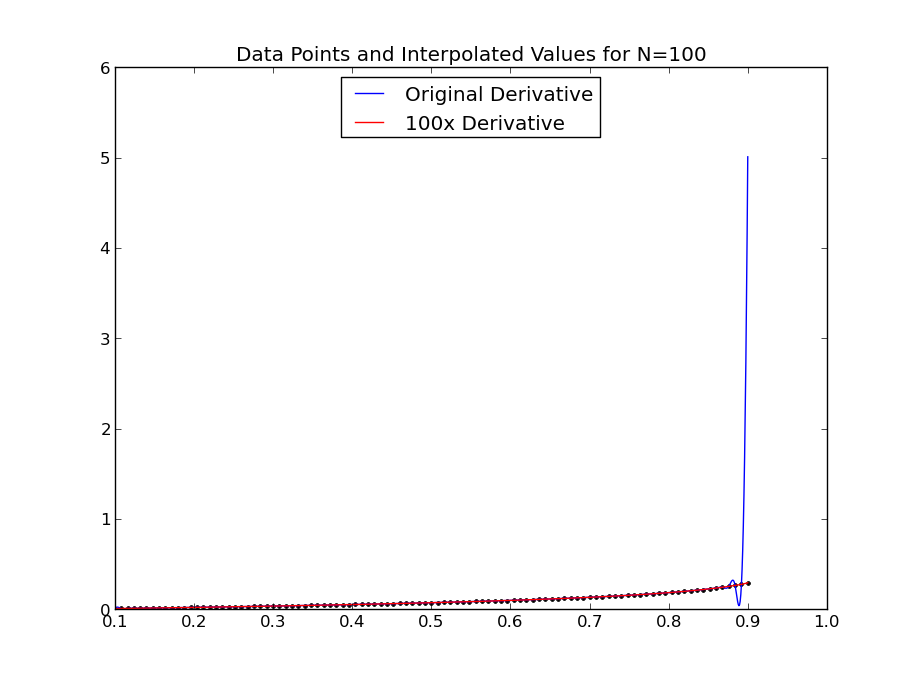
\includegraphics[width=\linewidth]{q5/func_comp.png}
                \caption{Interpolation for $N=100$}
                \label{fig:q5_func_comp}
                \end{subfigure}%
\begin{subfigure}{.5\textwidth}
  \centering
        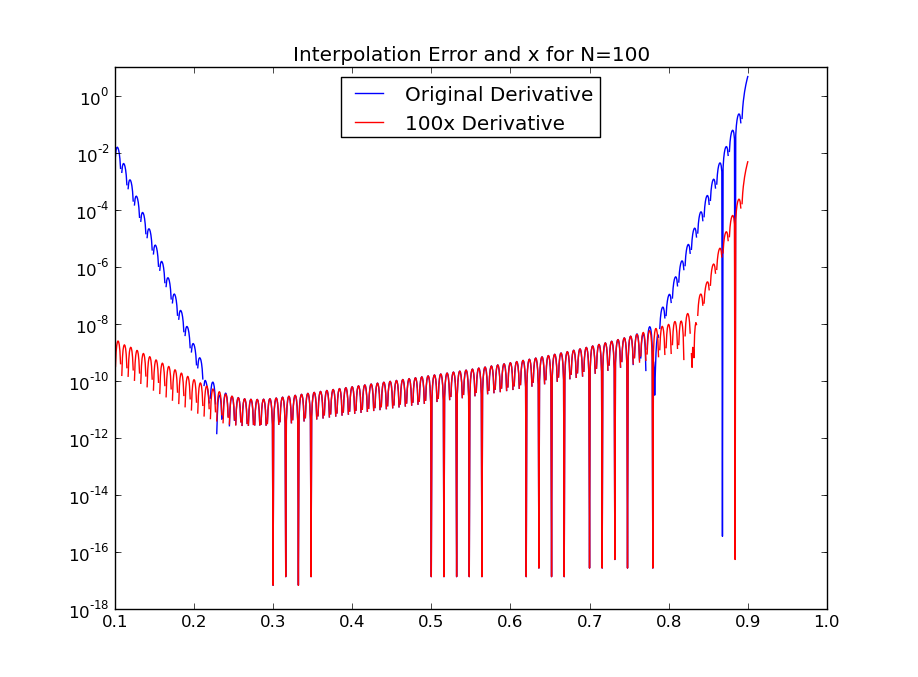
\includegraphics[width=\linewidth]{q5/err_comp.png}
                \caption{Spline Interpolation Error for $N=100$}
                \label{fig:q5_err_comp}
	\end{subfigure}
            
\caption{Cubic Spline Interpolation using $N=100$, using 100x thee actual derivative (compared with the original derivative)}
\label{fig:q5_1}        
\end{figure*}    


\pagebreak
\begin{figure*}
        \centering
        \begin{subfigure}{.5\textwidth}
  \centering
        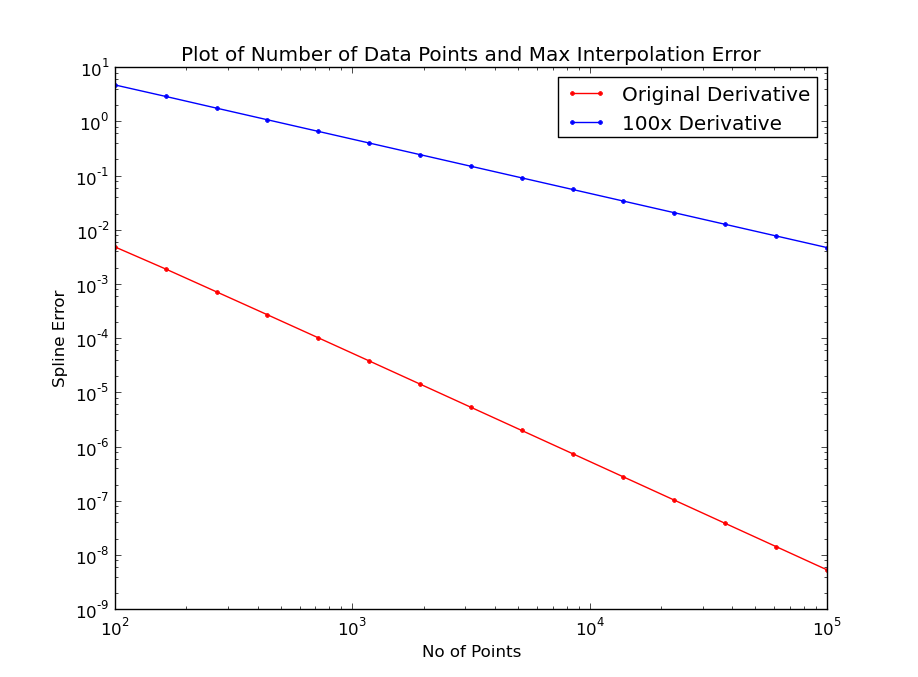
\includegraphics[width=\linewidth]{q5/loglogerr.png}
                \caption{Variation of Interpolation Error with Spacing}
                \label{fig:q5_loglogerr}
                \end{subfigure}%
\begin{subfigure}{.5\textwidth}
  \centering
        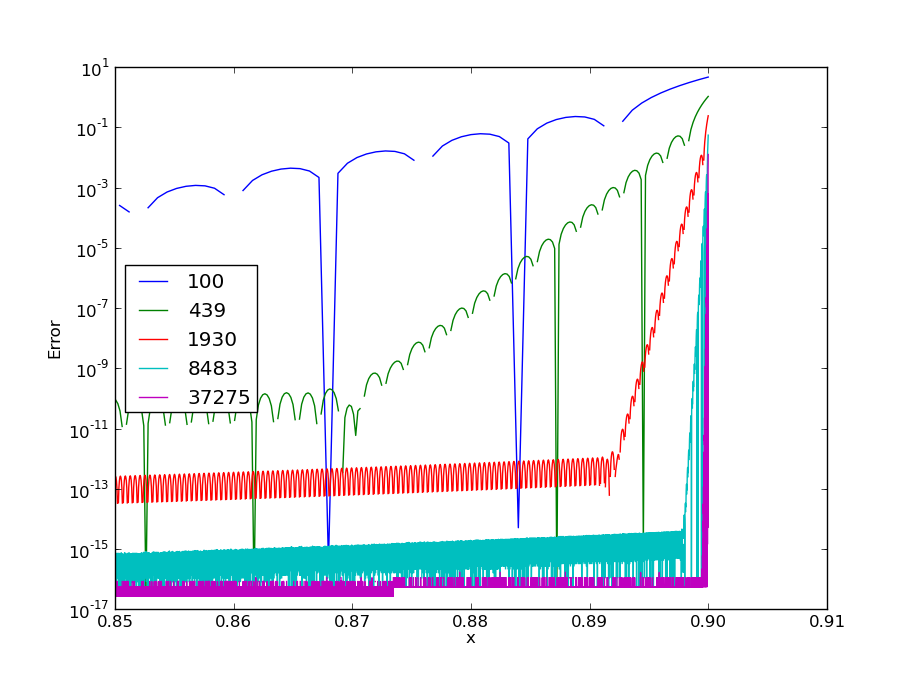
\includegraphics[width=\linewidth]{q5/err_vary.png}
                \caption{Focused variation with Spacing}
                \label{fig:q5_err_vary}
	\end{subfigure}
            
\caption{Variation of error with point spacing using $100$x the actual derivative, and the zoomed in error for $[0.85,0.9]$}
\label{fig:q5_2}        
\end{figure*}  

Figure (\ref{fig:q5_func_comp}) compares for interpolated function for using the original derivative values at $x=0.1,0.9$,  and $100$ times the actual value (using $N=100$ points). Figure (\ref{fig:q5_err_comp}) shows the error variation for the same. As we scale up the end point derivative, the error near the end points shoots up. But interestingly enough, the error in the middle regions (sufficiently far away from the edges) is \textbf{exactly} the same as using the theoretical derivative values. 

This means that somehow, the cubic spline tridiagonal matrix solver gives exactly the same 2nd-derivative values at the intermediate points, and it doesn't vary very much with the clamped derivative value. 

Figure (\ref{fig:q5_loglogerr}) shows the comparison of how the \textit{maximum}-error decays with the point spacing change. We see that using $100$x the derivative gives a strictly higher error decay. We see that using this, achieving 6-digit accuracy is not possible for similar order of points. There is an exponential scaling in the decay, but the \textsc{loglog} linear behaviour is maintained. 

Figure (\ref{fig:q5_err_vary}) shows how the error using $100$x derivative varies in $[0.85,0.9]$, that is near the singularity. As expected, the error is very high for low values of point spacing, and the error gets lower for lower point spacing. The spike in the error near $0.9$ is higher for a larger number of points, but the actual error is lower. 

\pagebreak


\question{6}{Question 6: Non-Uniform Spacing and Interpolation } 
\setcounter{section}{6}


\begin{figure}
\centering
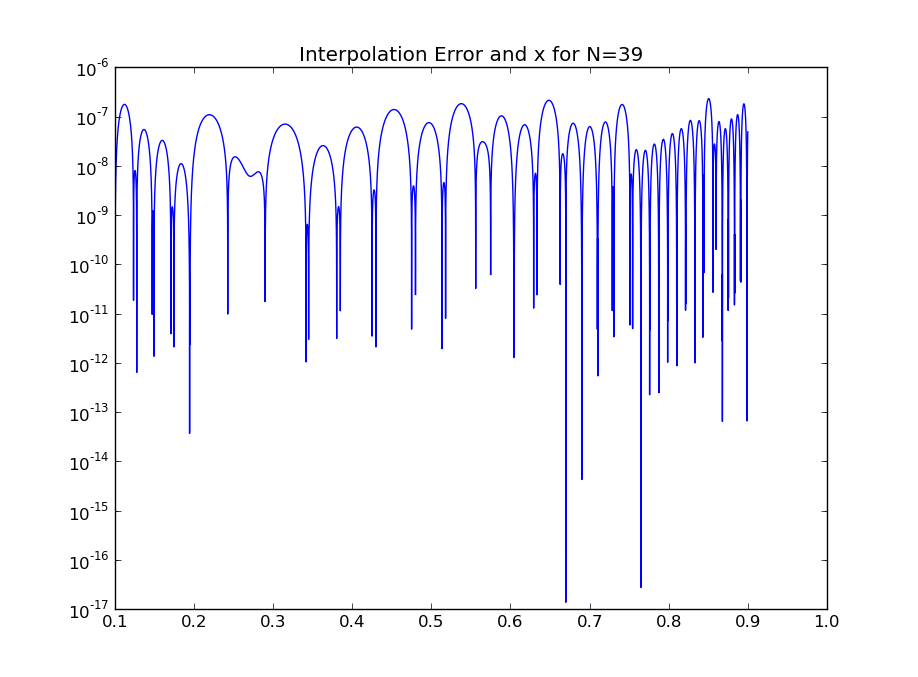
\includegraphics[width=0.6\linewidth]{q6/err.png}
\caption{Error variation using non-uniform spacing}
\label{fig:q6}
\vspace{-2.0em}
\end{figure}



In this section, we try to use non-uniform spacing to achieve 6-digit accuracy with the lowest number of data points. This means that we require a choice of points / spacing such that the error everywhere is strictly $< 10^{-6}$. 

In a very rough sense, the spline interpolation error grows as $\mathbb{O}(\frac{f^{(4)}(\zeta)}{4!}\Delta x^4)$, where $\zeta$ is chosen to maximize the 4th-derivative. This means that the interpolation error is upper bounded by the maximum value the 4th-derivative can take, and the the point-spacing raised to the 4th-power. We can use this to help achieve 6-digit accuracy.

Divide the range $[0.1,0.9]$ into windows of size say $w$ ($w=0.095$ was used). Now within each window, find the maximum value of the 4th-derivative (say at point $\zeta$). For some constant $c$ ($c=1$ was used), find $\Delta x$ such that

\begin{equation}
\frac{f^{(4)}(\zeta)}{4!}\Delta x^4 c < 10^{-6}
\end{equation}


\begin{wraptable}{r}{7.5cm}
\vspace{-1.5em}
\caption{Window and Number of sample points}
\renewcommand{\arraystretch}{1.0}
\label{tab:1}
\begin{tabular}{c|c} \toprule
Window interval & No of Sample points \\\midrule
0.100000 - 0.195000 & 5 \\
0.195000 - 0.290000 & 2 \\
0.290000 - 0.385000 & 2 \\
0.385000 - 0.480000 & 3 \\
0.480000 - 0.575000 & 3 \\
0.575000 - 0.670000 & 4 \\
0.670000 - 0.765000 & 5 \\
0.765000 - 0.860000 & 9 \\
0.860000 - 0.900000 & 6  \\\bottomrule
\end{tabular}
\end{wraptable}

Now sample the function within the window at this value of spacing $\Delta x$. Repeat this over all windows, and we have the sampled function.

An important design consideration here is the choice of the window size. If the window size is too small, we end up oversampling (as atleast one point is taken from each sample window). On the flip side, if the size of the sample window is too large and the derivative value is high in a window, the entire window is sampled at a very fine spacing (while it may not have been required for a smaller window size). We need to strike a fine balance between these 2. We found that with $c=1$ and a window spacing of $0.095$, we were able to achieve the required accuracy using just \textbf{39 sample points}. The number of points required in each interval are shown in Table (\ref{tab:1})


Figure (\ref{fig:q6}) shows how the error varies with $x$. We see an almost smooth peak variation, and the maximum interpolation error is about $2.4x10^{-7}$ using the $39$ point non-uniform sampling scheme. 

Note that it is possible to use an adaptive algorithm to come up with an even better point choice. It might be possible to combine points in the intervals further away from the singularity and maintain the accuracy. Our current point choice is fairly good since each interval has strictly more than 1 point. We chose $w=0.095$ so as to enable the last interval to be smaller, and thus the effects of high derivative is felt in the smaller interval. 

\question{7}{Question 7: Rational Interpolation } 
\setcounter{section}{7}
 
\begin{figure*}
\centering
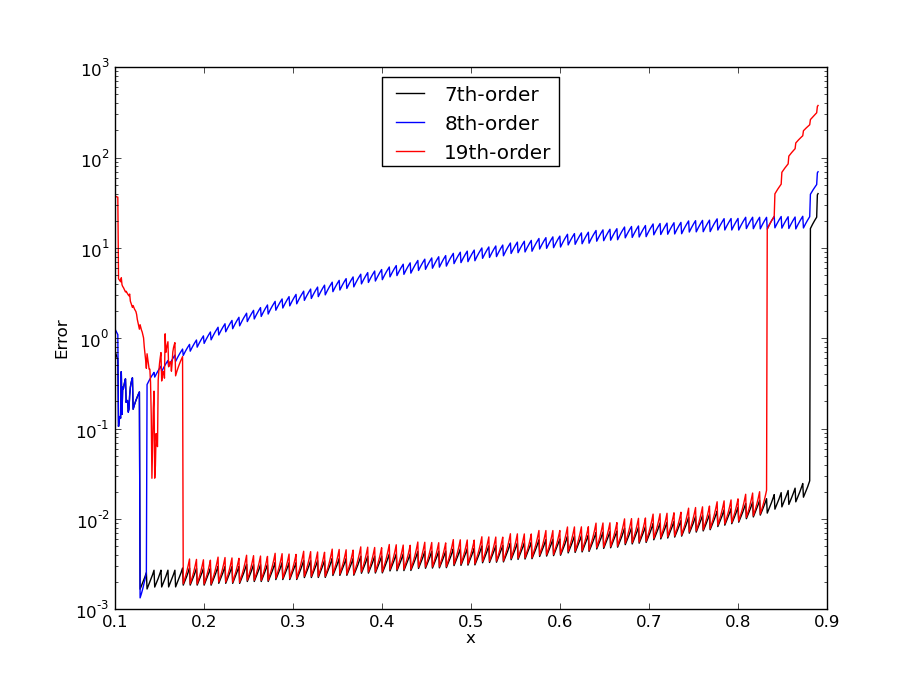
\includegraphics[width=0.6\linewidth]{q7/err_comp.png}
\caption{Error using Rational Interpolation, and variation with order}
\label{fig:q7}
\end{figure*}

In this section, we use rational interpolation on the function given above, and compare its performance to that of spline interpolation. Rational interpolation fits a rational polynomial to the function, of a specified maximum order. It is exceedingly useful in fitting functions with poles / which have rational semblance. Our given function is not exactly rational, but the interpolation should capture the pole behaviour quite well. We use ideas developed in \cite{NR}
 to write a Python script for rational interpolation, and thus fit it to the function. 

Figure (\ref{fig:q7}) shows the error variation for rational interpolation, and the order variation. The error for odd-order functions seems to be invariant of the order, indicating that it is well approximated by even a low order function. However, the interpolation value seems to blow up near the end points. Increasing the order doesn't seem to improve the best case performance. And the even-order rational interpolation seems to perform quite badly. As a whole, spline interpolation seems to do a lot better, and the error is more controllable. 

\pagebreak

\question{8}{Question 8: Two-Dimensional Interpolation } 
\setcounter{section}{8}
\setcounter{subsection}{0}

\begin{figure*}
        \centering
        \begin{subfigure}{.5\textwidth}
  \centering
        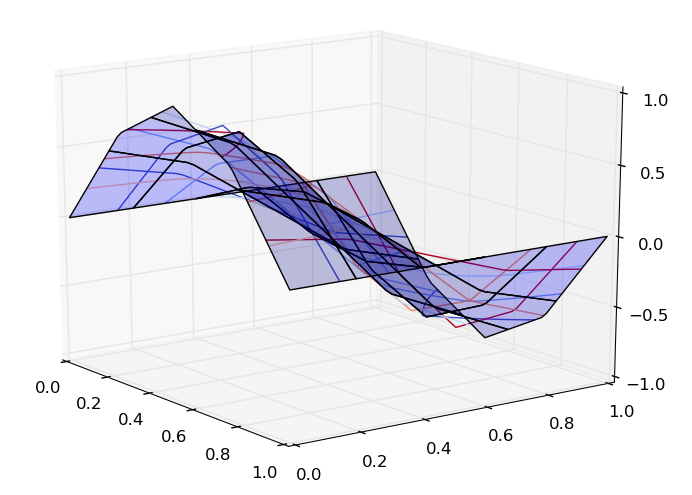
\includegraphics[width=1\linewidth]{q8/lin_func_5.png}
                \caption{Bilinear Interpolation function plot}
                \label{fig:q8_lin_func}
                \end{subfigure}%
\begin{subfigure}{.5\textwidth}
  \centering
        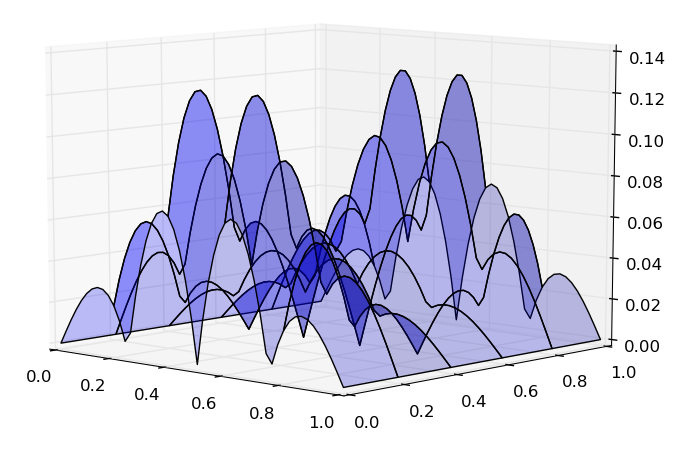
\includegraphics[width=1\linewidth]{q8/lin_err_5.png}
                \caption{Error in Bilinear interpolation}
                \label{fig:q8_lin_err}
	\end{subfigure}
            
\caption{Bilinear Interpolation function plot and error over the $50x50$ grid.}
\label{fig:q8_lin}        
\end{figure*}  

In this question, we analyse and compare various schemes of 2-dimensional interpolation. To do this, we create a $5x5$ grid of sample points for the smooth function
\begin{equation}
f(x,y) = sin(\pi x)cos(\pi y)
\end{equation}
in the range $[0,1]$ on both axes. This is a very well-behaved function, with known derivative values, so we use this as the testing ground for our algorithms. We want to interpolate to a $50x50$ mesh of points in the same interval. The various subsections to follow cover methods of interpolation, and how they compare.

\subsection{Bilinear interpolation}
Bilinear Interpolation is the most rudimentary interpolation scheme we consider here. In this scheme, for a given $(x,y)$ to be interpolated at, we consider the 4-nearest sample points $(x1,y1),(x1,y2),(x2,y2),(x2,y1)$ taken anti-clockwise from the bottom left ($x1<x2,y1<y2$). Let the function values at these points be $z11,z12,z22,z21$. Then the interpolated value is given by 
\begin{equation}
z=\frac{z11(x2-x)(y2-y)+z21(x-x1)(y2-y)}{(x2-x1)(y2-y1)}+\frac{z12(x2-x)(y-y1)+z22(x-x1)(y-y1)}{(x2-x1)(y2-y1)}
\end{equation}

This considers only the function value of the nearest 4 points and uses this to interpolate. We can easily see that this is only 2nd-order accurate in both the dimensions. 

Figure (\ref{fig:q8_lin_func}) shows a plot of the interpolated function (it resembles cos and sin projected on the axes). Figure (\ref{fig:q8_lin_err}) shows the plot of bilinear interpolation error. We see that the peak error is around $0.12$.

\pagebreak

\subsection{Bicubic Interpolation}

\begin{figure*}
        \centering
        \begin{subfigure}{.5\textwidth}
  \centering
        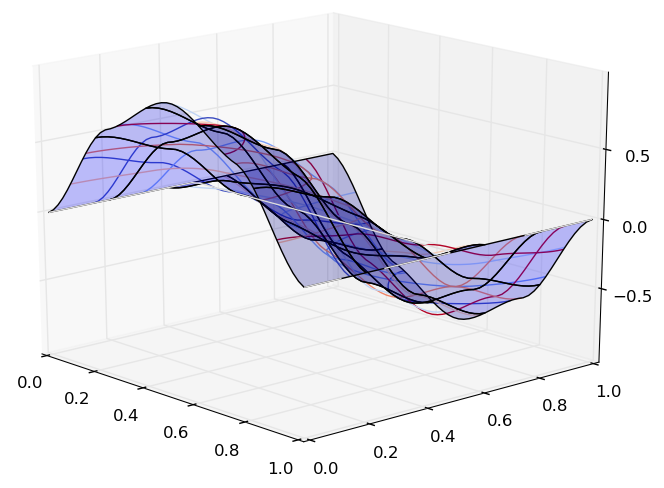
\includegraphics[width=1\linewidth]{q8/cubic_func_5.png}
                \caption{Bicubic Interpolation function plot}
                \label{fig:q8_cubic_func}
                \end{subfigure}%
\begin{subfigure}{.5\textwidth}
  \centering
        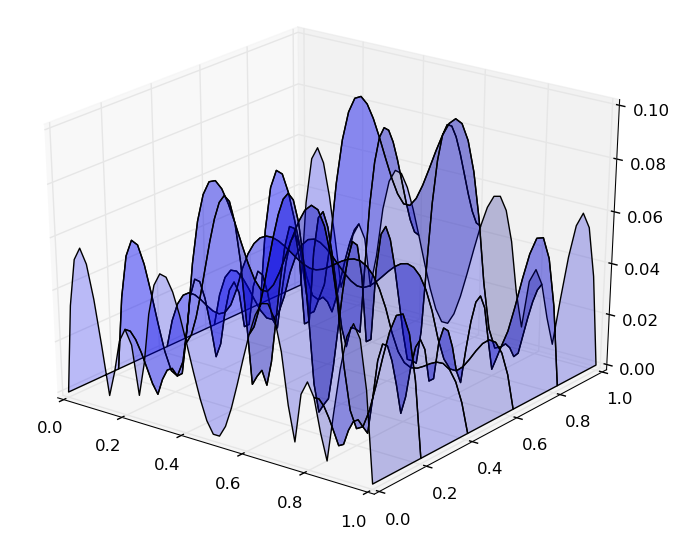
\includegraphics[width=1\linewidth]{q8/cubic_err_5.png}
                \caption{Error in Bicubic interpolation}
                \label{fig:q8_cubic_err}
	\end{subfigure}
            
\caption{Bicubic Interpolation function plot and error over the $50x50$ grid.}
\label{fig:q8_cubic}        
\end{figure*} 

Bicubic Interpolation aims at giving a piecewise smooth interpolation scheme. It requires the user to specify the derivatives at the 4 gridpoints (mentioned above), both the directional derivatives $\partial z/\partial x,\partial z/\partial y$ and the cross derivative $\partial^2 z/\partial x\partial y$. The exact interpolation scheme and the code from \cite{NR} was used for this question.

Figure (\ref{fig:q8_cubic_func}) shows a plot of the interpolated function (it resembles cos and sin projected on the axes). Figure (\ref{fig:q8_cubic_err}) shows the plot of bicubic interpolation error. We see that the peak error is around $0.08$, which is slightly than the linear interpolation error. The curve also a little smoother. 

We also plotted the behaviour of these 2 interpolation schemes using a 10x10 grid of sample points, and a 100x100 grid to be interpolated over, seen in Figures (\ref{fig:q8_lin_10}) and (\ref{fig:q8_cubic_10}). The results were quite different from the 5x5 case. Bilinear actually seemed to perform better in this case (peak error 0.015), and the error variation was a lot smoother than the bicubic interpolation (peak error 0.035). 

\begin{figure*}[h]
        \centering
        \begin{subfigure}{.5\textwidth}
  \centering
        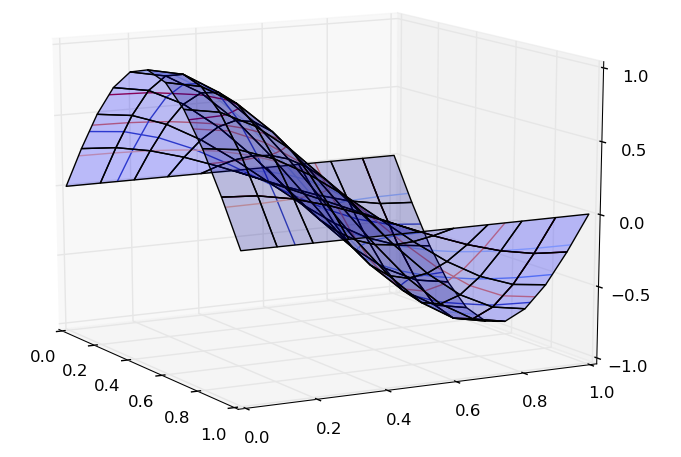
\includegraphics[width=1\linewidth]{q8/lin_func_10.png}
                \caption{Bilinear Interpolation function plot}
                \label{fig:q8_lin_func_10}
                \end{subfigure}%
\begin{subfigure}{.5\textwidth}
  \centering
        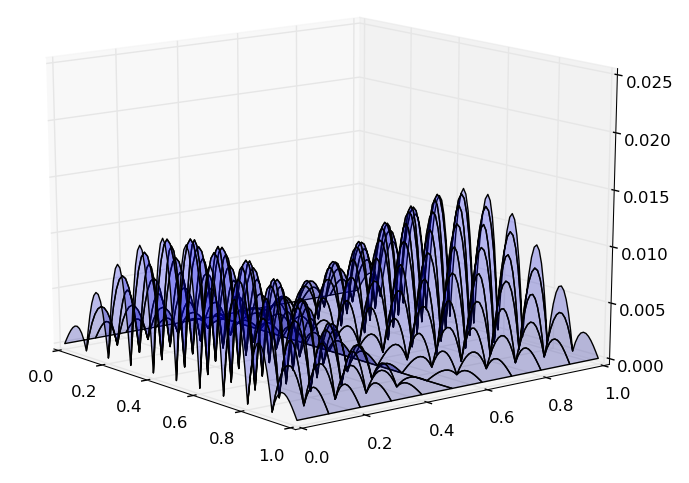
\includegraphics[width=1\linewidth]{q8/lin_err_10.png}
                \caption{Error in Bilinear interpolation}
                \label{fig:q8_lin_err_10}
	\end{subfigure}
            
\caption{Bilinear Interpolation function plot and error over the 100x100 grid.}
\label{fig:q8_lin_10}        
\end{figure*}  

\begin{figure*}[h]
        \centering
        \begin{subfigure}{.5\textwidth}
  \centering
        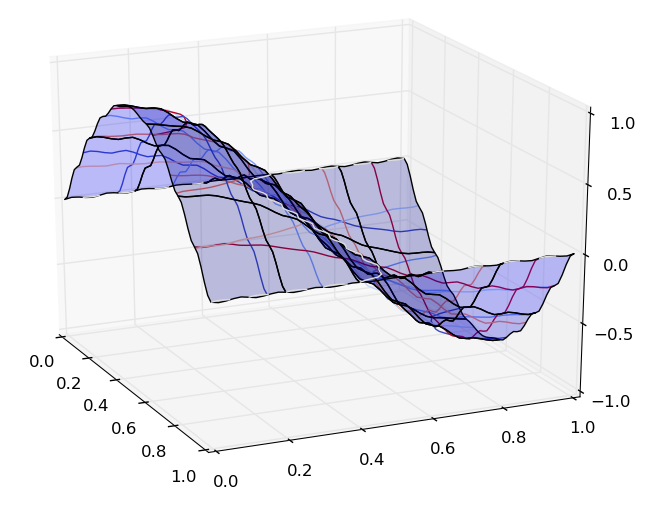
\includegraphics[width=1\linewidth]{q8/cubic_func_10.png}
                \caption{Bicubic Interpolation function plot}
                \label{fig:q8_cubic_func_10}
                \end{subfigure}%
\begin{subfigure}{.5\textwidth}
  \centering
        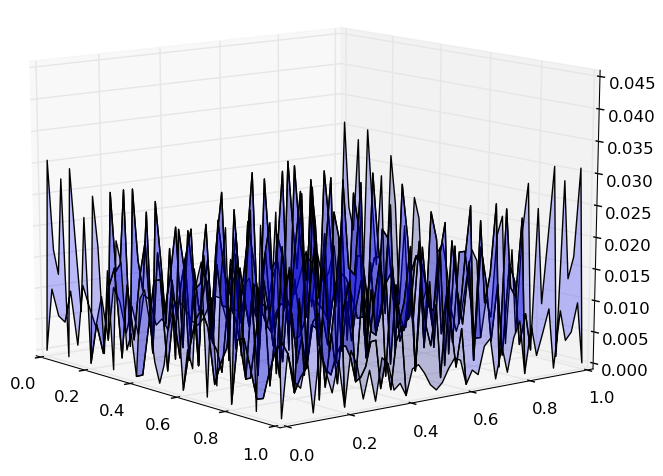
\includegraphics[width=1\linewidth]{q8/cubic_err_10.png}
                \caption{Error in Bicubic interpolation}
                \label{fig:q8_cubic_err_10}
	\end{subfigure}
            
\caption{Bicubic Interpolation function plot and error over the 100x100 grid.}
\label{fig:q8_cubic_10}        
\end{figure*} 


\begin{thebibliography}{155}
\bibitem{NR}
William H. Press, Saul A. Teukolsky, William T. Vetterling, Brian P. Flannery, "Numerical Recipes in C" 

\bibitem{Stoer}
J. Stoer, R. Bulirsch, "Introduction to Numerical Analysis"

\end{thebibliography}


\end{document}